\section{Approach}	\label{sec:related_works}

The algorithmic structure of MABDI can be seen in Fig. \ref{fig:system}. The diagram is very similar to Fig. \ref{fig:pipeline} with the exception of the Classification component, shown in blue. This Classification component is MABDI's contribution to the state-of-art in mesh based mapping algorithms, and is what gives MABDI the ability to make decisions about the incoming data.

The Classification component consists of two elements:
\begin{enumerate}
    \item \textit{Generate Expected Depth Image $E$} - Here we take the global
    mesh $M$, render it using computer graphics, and use the depth buffer of the
    render window to create a depth image $E$ of what we expect to see from our
    sensor. This method requires the current pose $P$ of the actual sensor
    (simulated for our experiments).
    \item \textit{Classify Depth Image $D$} - Here we classify the actual depth
    image $D$ (simulated for our experiments) by first taking the absolute
    difference between $E$ and $D$ and thresholding. If the differences are
    small, those points are thrown away and if the differences are large, those
    points are kept as $D_n$. The idea behind this is, if the difference is
    large, the measurements are coming from a part of the environment that has
    not been seen before i.e. novel. The implication of is assumption, is that
    this version of MABDI can not handle object removal. It is worth noting,
    that MABDI can be extended to handle object removal by using the sign of the
    difference between $E$ and $D$ instead of the absolute value.
\end{enumerate}

\begin{figure}[h]%[thpb]
\centering
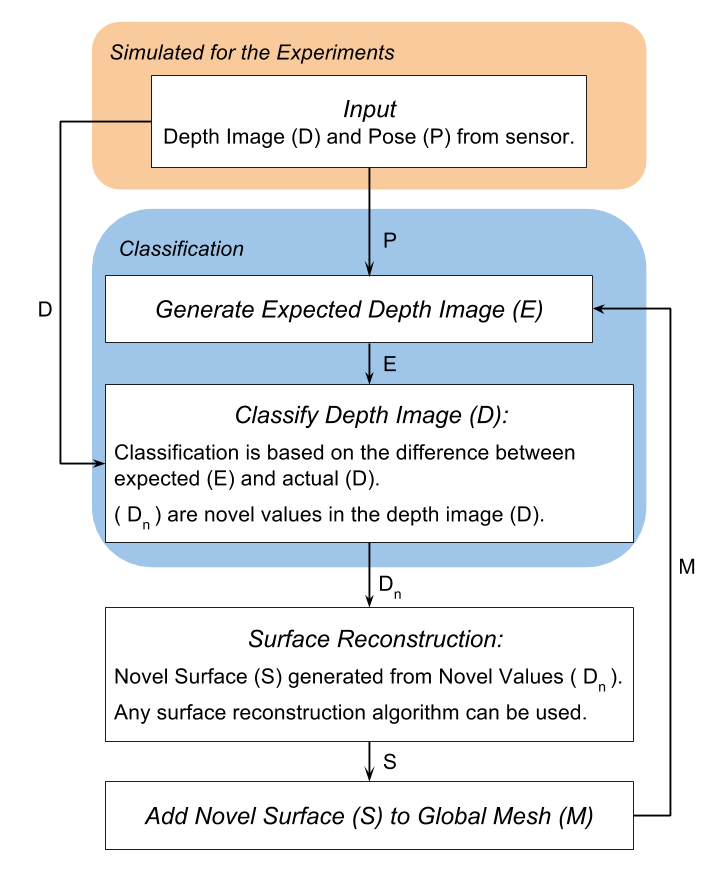
\includegraphics[width=.5\textwidth]{figures/diagram_system.png}
\caption{MABDI system diagram}
\label{fig:system}
\end{figure}



\begin{figure}[h]%[thpb]
\centering
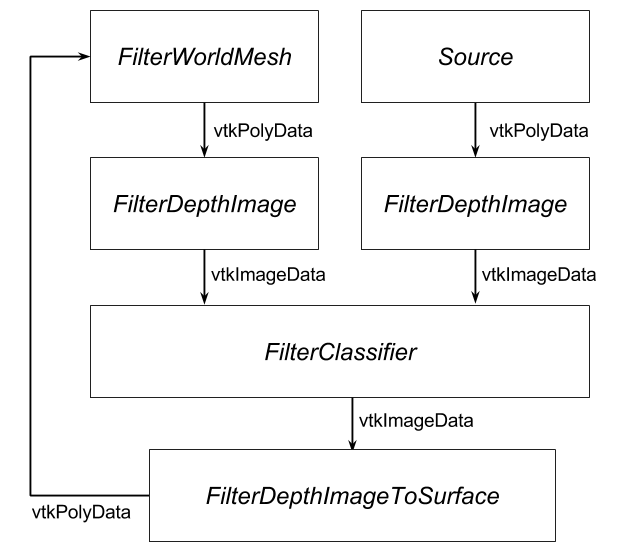
\includegraphics[width=.5\textwidth]{figures/diagram_software.png}
\caption{MABDI software diagram}
\label{fig:software}
\end{figure}
